\documentclass[twoside]{book}

% Packages required by doxygen
\usepackage{fixltx2e}
\usepackage{calc}
\usepackage{doxygen}
\usepackage[export]{adjustbox} % also loads graphicx
\usepackage{graphicx}
\usepackage[utf8]{inputenc}
\usepackage{makeidx}
\usepackage{multicol}
\usepackage{multirow}
\PassOptionsToPackage{warn}{textcomp}
\usepackage{textcomp}
\usepackage[nointegrals]{wasysym}
\usepackage[table]{xcolor}

% Font selection
\usepackage[T1]{fontenc}
\usepackage[scaled=.90]{helvet}
\usepackage{courier}
\usepackage{amssymb}
\usepackage{sectsty}
\renewcommand{\familydefault}{\sfdefault}
\allsectionsfont{%
  \fontseries{bc}\selectfont%
  \color{darkgray}%
}
\renewcommand{\DoxyLabelFont}{%
  \fontseries{bc}\selectfont%
  \color{darkgray}%
}
\newcommand{\+}{\discretionary{\mbox{\scriptsize$\hookleftarrow$}}{}{}}

% Page & text layout
\usepackage{geometry}
\geometry{%
  a4paper,%
  top=2.5cm,%
  bottom=2.5cm,%
  left=2.5cm,%
  right=2.5cm%
}
\tolerance=750
\hfuzz=15pt
\hbadness=750
\setlength{\emergencystretch}{15pt}
\setlength{\parindent}{0cm}
\setlength{\parskip}{3ex plus 2ex minus 2ex}
\makeatletter
\renewcommand{\paragraph}{%
  \@startsection{paragraph}{4}{0ex}{-1.0ex}{1.0ex}{%
    \normalfont\normalsize\bfseries\SS@parafont%
  }%
}
\renewcommand{\subparagraph}{%
  \@startsection{subparagraph}{5}{0ex}{-1.0ex}{1.0ex}{%
    \normalfont\normalsize\bfseries\SS@subparafont%
  }%
}
\makeatother

% Headers & footers
\usepackage{fancyhdr}
\pagestyle{fancyplain}
\fancyhead[LE]{\fancyplain{}{\bfseries\thepage}}
\fancyhead[CE]{\fancyplain{}{}}
\fancyhead[RE]{\fancyplain{}{\bfseries\leftmark}}
\fancyhead[LO]{\fancyplain{}{\bfseries\rightmark}}
\fancyhead[CO]{\fancyplain{}{}}
\fancyhead[RO]{\fancyplain{}{\bfseries\thepage}}
\fancyfoot[LE]{\fancyplain{}{}}
\fancyfoot[CE]{\fancyplain{}{}}
\fancyfoot[RE]{\fancyplain{}{\bfseries\scriptsize Generated by Doxygen }}
\fancyfoot[LO]{\fancyplain{}{\bfseries\scriptsize Generated by Doxygen }}
\fancyfoot[CO]{\fancyplain{}{}}
\fancyfoot[RO]{\fancyplain{}{}}
\renewcommand{\footrulewidth}{0.4pt}
\renewcommand{\chaptermark}[1]{%
  \markboth{#1}{}%
}
\renewcommand{\sectionmark}[1]{%
  \markright{\thesection\ #1}%
}

% Indices & bibliography
\usepackage{natbib}
\usepackage[titles]{tocloft}
\setcounter{tocdepth}{3}
\setcounter{secnumdepth}{5}
\makeindex

% Hyperlinks (required, but should be loaded last)
\usepackage{ifpdf}
\ifpdf
  \usepackage[pdftex,pagebackref=true]{hyperref}
\else
  \usepackage[ps2pdf,pagebackref=true]{hyperref}
\fi
\hypersetup{%
  colorlinks=true,%
  linkcolor=blue,%
  citecolor=blue,%
  unicode%
}

% Custom commands
\newcommand{\clearemptydoublepage}{%
  \newpage{\pagestyle{empty}\cleardoublepage}%
}

\usepackage{caption}
\captionsetup{labelsep=space,justification=centering,font={bf},singlelinecheck=off,skip=4pt,position=top}

%===== C O N T E N T S =====

\begin{document}

% Titlepage & ToC
\hypersetup{pageanchor=false,
             bookmarksnumbered=true,
             pdfencoding=unicode
            }
\pagenumbering{alph}
\begin{titlepage}
\vspace*{7cm}
\begin{center}%
{\Large My Project }\\
\vspace*{1cm}
{\large Generated by Doxygen 1.8.13}\\
\end{center}
\end{titlepage}
\clearemptydoublepage
\pagenumbering{roman}
\tableofcontents
\clearemptydoublepage
\pagenumbering{arabic}
\hypersetup{pageanchor=true}

%--- Begin generated contents ---
\chapter{Main Page}
\label{index}\hypertarget{index}{}En el siguiente .cpp se demuestra una forma en la que se puede programar un M\+S\+T-\/coloreado para que esta cumpla las mismas funciones que el original con la nueva condicional de los colores.


\begin{DoxyItemize}
\item Haciendo uso de los temas realizados durante el semestre
\item Incluyendo una librería de salida y entrada de archivos para graficar.
\item Incluyendo la librería algorithm para poder usar las distintas funciones 
\end{DoxyItemize}
\chapter{Class Index}
\section{Class List}
Here are the classes, structs, unions and interfaces with brief descriptions\+:\begin{DoxyCompactList}
\item\contentsline{section}{\hyperlink{structEdge}{Edge} \\*Representa la estructura de las aristas  Contiene los datos miembros de la arista, una funcion para condicionar el sort }{\pageref{structEdge}}{}
\end{DoxyCompactList}

\chapter{File Index}
\section{File List}
Here is a list of all documented files with brief descriptions\+:\begin{DoxyCompactList}
\item\contentsline{section}{\hyperlink{MiniColST_8cpp}{Mini\+Col\+S\+T.\+cpp} \\*Implementacion del un M\+S\+T-\/coloreado en C++ }{\pageref{MiniColST_8cpp}}{}
\end{DoxyCompactList}

\chapter{Class Documentation}
\hypertarget{structEdge}{}\section{Edge Struct Reference}
\label{structEdge}\index{Edge@{Edge}}


Representa la estructura de las aristas  Contiene los datos miembros de la arista, una funcion para condicionar el sort.  


\subsection*{Public Member Functions}
\begin{DoxyCompactItemize}
\item 
\mbox{\Hypertarget{structEdge_ac9199551fe9afee1b079b9d434068532}\label{structEdge_ac9199551fe9afee1b079b9d434068532}} 
bool {\bfseries operator$<$} (const \hyperlink{structEdge}{Edge} \&e) const
\end{DoxyCompactItemize}
\subsection*{Public Attributes}
\begin{DoxyCompactItemize}
\item 
\mbox{\Hypertarget{structEdge_a7db302e155f6b91b908ee4ffd9d37331}\label{structEdge_a7db302e155f6b91b908ee4ffd9d37331}} 
int {\bfseries orig}
\item 
\mbox{\Hypertarget{structEdge_ad7df434ff7710e69f28bb31e91a35f82}\label{structEdge_ad7df434ff7710e69f28bb31e91a35f82}} 
int {\bfseries dest}
\item 
\mbox{\Hypertarget{structEdge_a95aba41a052cf8787107f8ca000fd8e6}\label{structEdge_a95aba41a052cf8787107f8ca000fd8e6}} 
int {\bfseries peso}
\item 
\mbox{\Hypertarget{structEdge_a7bdb4667054bb53fe27a9438bb6b2b42}\label{structEdge_a7bdb4667054bb53fe27a9438bb6b2b42}} 
char {\bfseries color}
\item 
\mbox{\Hypertarget{structEdge_a76d10f80be295bbdb4ff0a55839c31b0}\label{structEdge_a76d10f80be295bbdb4ff0a55839c31b0}} 
bool {\bfseries flag}
\end{DoxyCompactItemize}


\subsection{Detailed Description}
Representa la estructura de las aristas  Contiene los datos miembros de la arista, una funcion para condicionar el sort. 

The documentation for this struct was generated from the following file\+:\begin{DoxyCompactItemize}
\item 
\hyperlink{MiniColST_8cpp}{Mini\+Col\+S\+T.\+cpp}\end{DoxyCompactItemize}

\chapter{File Documentation}
\hypertarget{MiniColST_8cpp}{}\section{Mini\+Col\+S\+T.\+cpp File Reference}
\label{MiniColST_8cpp}\index{Mini\+Col\+S\+T.\+cpp@{Mini\+Col\+S\+T.\+cpp}}


implementacion del un M\+S\+T-\/coloreado en C++.  


{\ttfamily \#include $<$iostream$>$}\newline
{\ttfamily \#include $<$algorithm$>$}\newline
{\ttfamily \#include $<$stdio.\+h$>$}\newline
{\ttfamily \#include $<$cstring$>$}\newline
{\ttfamily \#include $<$fstream$>$}\newline
Include dependency graph for Mini\+Col\+S\+T.\+cpp\+:
\nopagebreak
\begin{figure}[H]
\begin{center}
\leavevmode
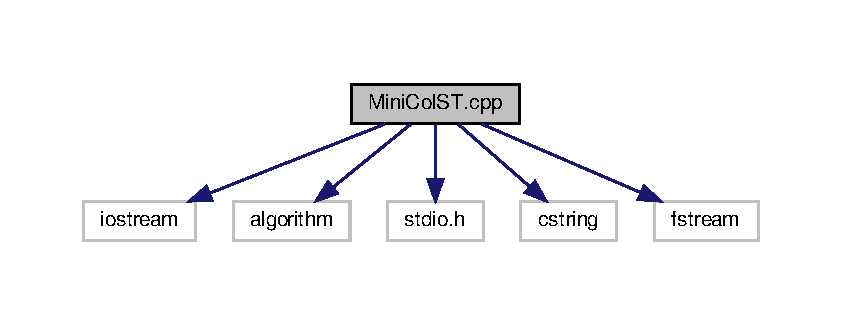
\includegraphics[width=350pt]{MiniColST_8cpp__incl}
\end{center}
\end{figure}
\subsection*{Classes}
\begin{DoxyCompactItemize}
\item 
struct \hyperlink{structEdge}{Edge}
\begin{DoxyCompactList}\small\item\em Representa la estructura de las aristas  Contiene los datos miembros de la arista, una funcion para condicionar el sort. \end{DoxyCompactList}\end{DoxyCompactItemize}
\subsection*{Macros}
\begin{DoxyCompactItemize}
\item 
\mbox{\Hypertarget{MiniColST_8cpp_a392fb874e547e582e9c66a08a1f23326}\label{MiniColST_8cpp_a392fb874e547e582e9c66a08a1f23326}} 
\#define {\bfseries M\+AX}~1005
\end{DoxyCompactItemize}
\subsection*{Functions}
\begin{DoxyCompactItemize}
\item 
void \hyperlink{MiniColST_8cpp_af9f028303a1e74b3a20363a7f30f915f}{Make\+Set} (int n)
\item 
int \hyperlink{MiniColST_8cpp_a34b9ead0608e676d9ae5188672427cc8}{Find} (int x)
\item 
void \hyperlink{MiniColST_8cpp_a44481bb75386fbb0f958a388d4b9f757}{Union} (int x, int y)
\item 
bool \hyperlink{MiniColST_8cpp_a44619b6f7489e5097190700c5abb59ea}{Ciclo} (int x, int y)
\item 
void \hyperlink{MiniColST_8cpp_a63e25b3dc17c382ae0a47f9078f17a1b}{print\+Grafo} (\hyperlink{structEdge}{Edge} M\+ST\mbox{[}$\,$\mbox{]}, int num)
\item 
void \hyperlink{MiniColST_8cpp_ae6d9fb6b62bf4b3c3d9435def5f21fd1}{printG} (\hyperlink{structEdge}{Edge} M\+ST\mbox{[}$\,$\mbox{]}, int num)
\item 
void \hyperlink{MiniColST_8cpp_aa991861816692223e6221a4008c04985}{Kruskal\+Aristas\+Azules} (int n)
\item 
void \hyperlink{MiniColST_8cpp_a58419a35198a8fa1fda3cedbf764d218}{Kruskal\+Max\+Aristas\+Azules} ()
\item 
void \hyperlink{MiniColST_8cpp_a46888dccd7273a2eb1e3e7fa251b72d6}{Kruskal\+Min\+Aristas\+Azules} ()
\item 
void \hyperlink{MiniColST_8cpp_a979ac68eb2ed97aef6cfa7c45fc1c8f0}{Aristas\+Azules} ()
\item 
void \hyperlink{MiniColST_8cpp_a140c4d775cfd71981c254c354ca191a5}{Max\+Min\+Aristas\+Azules} (int select)
\item 
void \hyperlink{MiniColST_8cpp_a02fd73d861ef2e4aabb38c0c9ff82947}{init} ()
\item 
int \hyperlink{MiniColST_8cpp_ae66f6b31b5ad750f1fe042a706a4e3d4}{main} ()
\end{DoxyCompactItemize}
\subsection*{Variables}
\begin{DoxyCompactItemize}
\item 
\mbox{\Hypertarget{MiniColST_8cpp_ab0345f76d1ddceda1a4a3f8dd8edbbe5}\label{MiniColST_8cpp_ab0345f76d1ddceda1a4a3f8dd8edbbe5}} 
int {\bfseries Parent} \mbox{[}M\+AX\mbox{]}
\item 
\mbox{\Hypertarget{MiniColST_8cpp_a91e334f289dc11ba09da0df4a9c72123}\label{MiniColST_8cpp_a91e334f289dc11ba09da0df4a9c72123}} 
int {\bfseries V}
\item 
\mbox{\Hypertarget{MiniColST_8cpp_a105a63272424d04208f33bac739acf98}\label{MiniColST_8cpp_a105a63272424d04208f33bac739acf98}} 
int {\bfseries E}
\item 
\mbox{\Hypertarget{MiniColST_8cpp_ac22944fb3ead4c2f75cc37214b24761d}\label{MiniColST_8cpp_ac22944fb3ead4c2f75cc37214b24761d}} 
struct \hyperlink{structEdge}{Edge} {\bfseries arista} \mbox{[}M\+AX\mbox{]}
\item 
\mbox{\Hypertarget{MiniColST_8cpp_af7c9fc6fb71de935b6f606ee4d8a9bb0}\label{MiniColST_8cpp_af7c9fc6fb71de935b6f606ee4d8a9bb0}} 
\hyperlink{structEdge}{Edge} {\bfseries M\+ST} \mbox{[}M\+AX\mbox{]}
\end{DoxyCompactItemize}


\subsection{Detailed Description}
implementacion del un M\+S\+T-\/coloreado en C++. 

\begin{DoxyAuthor}{Author}
i\+Mawe 
\end{DoxyAuthor}
\begin{DoxyVersion}{Version}
Revision 1.\+1 
\end{DoxyVersion}


\subsection{Function Documentation}
\mbox{\Hypertarget{MiniColST_8cpp_a979ac68eb2ed97aef6cfa7c45fc1c8f0}\label{MiniColST_8cpp_a979ac68eb2ed97aef6cfa7c45fc1c8f0}} 
\index{Mini\+Col\+S\+T.\+cpp@{Mini\+Col\+S\+T.\+cpp}!Aristas\+Azules@{Aristas\+Azules}}
\index{Aristas\+Azules@{Aristas\+Azules}!Mini\+Col\+S\+T.\+cpp@{Mini\+Col\+S\+T.\+cpp}}
\subsubsection{\texorpdfstring{Aristas\+Azules()}{AristasAzules()}}
{\footnotesize\ttfamily void Aristas\+Azules (\begin{DoxyParamCaption}{ }\end{DoxyParamCaption})}

Funcion para llamar a M\+ST segun k aristas azules. \mbox{\Hypertarget{MiniColST_8cpp_a44619b6f7489e5097190700c5abb59ea}\label{MiniColST_8cpp_a44619b6f7489e5097190700c5abb59ea}} 
\index{Mini\+Col\+S\+T.\+cpp@{Mini\+Col\+S\+T.\+cpp}!Ciclo@{Ciclo}}
\index{Ciclo@{Ciclo}!Mini\+Col\+S\+T.\+cpp@{Mini\+Col\+S\+T.\+cpp}}
\subsubsection{\texorpdfstring{Ciclo()}{Ciclo()}}
{\footnotesize\ttfamily bool Ciclo (\begin{DoxyParamCaption}\item[{int}]{x,  }\item[{int}]{y }\end{DoxyParamCaption})}

Funcion para verificar si existe un ciclo. 
\begin{DoxyParams}{Parameters}
{\em x,y,son} & los vertices los cuales se van a comparar si forman un ciclo. \\
\hline
\end{DoxyParams}
\mbox{\Hypertarget{MiniColST_8cpp_a34b9ead0608e676d9ae5188672427cc8}\label{MiniColST_8cpp_a34b9ead0608e676d9ae5188672427cc8}} 
\index{Mini\+Col\+S\+T.\+cpp@{Mini\+Col\+S\+T.\+cpp}!Find@{Find}}
\index{Find@{Find}!Mini\+Col\+S\+T.\+cpp@{Mini\+Col\+S\+T.\+cpp}}
\subsubsection{\texorpdfstring{Find()}{Find()}}
{\footnotesize\ttfamily int Find (\begin{DoxyParamCaption}\item[{int}]{x }\end{DoxyParamCaption})}

Funcion para buscar la raiz. 
\begin{DoxyParams}{Parameters}
{\em c,se} & envia el nodo a buscar \\
\hline
\end{DoxyParams}
\mbox{\Hypertarget{MiniColST_8cpp_a02fd73d861ef2e4aabb38c0c9ff82947}\label{MiniColST_8cpp_a02fd73d861ef2e4aabb38c0c9ff82947}} 
\index{Mini\+Col\+S\+T.\+cpp@{Mini\+Col\+S\+T.\+cpp}!init@{init}}
\index{init@{init}!Mini\+Col\+S\+T.\+cpp@{Mini\+Col\+S\+T.\+cpp}}
\subsubsection{\texorpdfstring{init()}{init()}}
{\footnotesize\ttfamily void init (\begin{DoxyParamCaption}{ }\end{DoxyParamCaption})}

Funcion para iniciar el programa para realizar el M\+S\+T-\/\+Coloreado. \mbox{\Hypertarget{MiniColST_8cpp_aa991861816692223e6221a4008c04985}\label{MiniColST_8cpp_aa991861816692223e6221a4008c04985}} 
\index{Mini\+Col\+S\+T.\+cpp@{Mini\+Col\+S\+T.\+cpp}!Kruskal\+Aristas\+Azules@{Kruskal\+Aristas\+Azules}}
\index{Kruskal\+Aristas\+Azules@{Kruskal\+Aristas\+Azules}!Mini\+Col\+S\+T.\+cpp@{Mini\+Col\+S\+T.\+cpp}}
\subsubsection{\texorpdfstring{Kruskal\+Aristas\+Azules()}{KruskalAristasAzules()}}
{\footnotesize\ttfamily void Kruskal\+Aristas\+Azules (\begin{DoxyParamCaption}\item[{int}]{n }\end{DoxyParamCaption})}

Funcion para hallar M\+ST con k aristas azules. 
\begin{DoxyParams}{Parameters}
{\em n,el} & numero de aristas que tiene el M\+ST \\
\hline
\end{DoxyParams}
\mbox{\Hypertarget{MiniColST_8cpp_a58419a35198a8fa1fda3cedbf764d218}\label{MiniColST_8cpp_a58419a35198a8fa1fda3cedbf764d218}} 
\index{Mini\+Col\+S\+T.\+cpp@{Mini\+Col\+S\+T.\+cpp}!Kruskal\+Max\+Aristas\+Azules@{Kruskal\+Max\+Aristas\+Azules}}
\index{Kruskal\+Max\+Aristas\+Azules@{Kruskal\+Max\+Aristas\+Azules}!Mini\+Col\+S\+T.\+cpp@{Mini\+Col\+S\+T.\+cpp}}
\subsubsection{\texorpdfstring{Kruskal\+Max\+Aristas\+Azules()}{KruskalMaxAristasAzules()}}
{\footnotesize\ttfamily void Kruskal\+Max\+Aristas\+Azules (\begin{DoxyParamCaption}{ }\end{DoxyParamCaption})}

Funcion para hallar M\+ST con el numero maximo aristas azules. \mbox{\Hypertarget{MiniColST_8cpp_a46888dccd7273a2eb1e3e7fa251b72d6}\label{MiniColST_8cpp_a46888dccd7273a2eb1e3e7fa251b72d6}} 
\index{Mini\+Col\+S\+T.\+cpp@{Mini\+Col\+S\+T.\+cpp}!Kruskal\+Min\+Aristas\+Azules@{Kruskal\+Min\+Aristas\+Azules}}
\index{Kruskal\+Min\+Aristas\+Azules@{Kruskal\+Min\+Aristas\+Azules}!Mini\+Col\+S\+T.\+cpp@{Mini\+Col\+S\+T.\+cpp}}
\subsubsection{\texorpdfstring{Kruskal\+Min\+Aristas\+Azules()}{KruskalMinAristasAzules()}}
{\footnotesize\ttfamily void Kruskal\+Min\+Aristas\+Azules (\begin{DoxyParamCaption}{ }\end{DoxyParamCaption})}

Funcion para hallar M\+ST con el numero minimo aristas azules. \mbox{\Hypertarget{MiniColST_8cpp_ae66f6b31b5ad750f1fe042a706a4e3d4}\label{MiniColST_8cpp_ae66f6b31b5ad750f1fe042a706a4e3d4}} 
\index{Mini\+Col\+S\+T.\+cpp@{Mini\+Col\+S\+T.\+cpp}!main@{main}}
\index{main@{main}!Mini\+Col\+S\+T.\+cpp@{Mini\+Col\+S\+T.\+cpp}}
\subsubsection{\texorpdfstring{main()}{main()}}
{\footnotesize\ttfamily int main (\begin{DoxyParamCaption}{ }\end{DoxyParamCaption})}

Funcion Main. \mbox{\Hypertarget{MiniColST_8cpp_af9f028303a1e74b3a20363a7f30f915f}\label{MiniColST_8cpp_af9f028303a1e74b3a20363a7f30f915f}} 
\index{Mini\+Col\+S\+T.\+cpp@{Mini\+Col\+S\+T.\+cpp}!Make\+Set@{Make\+Set}}
\index{Make\+Set@{Make\+Set}!Mini\+Col\+S\+T.\+cpp@{Mini\+Col\+S\+T.\+cpp}}
\subsubsection{\texorpdfstring{Make\+Set()}{MakeSet()}}
{\footnotesize\ttfamily void Make\+Set (\begin{DoxyParamCaption}\item[{int}]{n }\end{DoxyParamCaption})}

Funcion crear los pares. 
\begin{DoxyParams}{Parameters}
{\em n,se} & envia el numero de vertices \\
\hline
\end{DoxyParams}
\mbox{\Hypertarget{MiniColST_8cpp_a140c4d775cfd71981c254c354ca191a5}\label{MiniColST_8cpp_a140c4d775cfd71981c254c354ca191a5}} 
\index{Mini\+Col\+S\+T.\+cpp@{Mini\+Col\+S\+T.\+cpp}!Max\+Min\+Aristas\+Azules@{Max\+Min\+Aristas\+Azules}}
\index{Max\+Min\+Aristas\+Azules@{Max\+Min\+Aristas\+Azules}!Mini\+Col\+S\+T.\+cpp@{Mini\+Col\+S\+T.\+cpp}}
\subsubsection{\texorpdfstring{Max\+Min\+Aristas\+Azules()}{MaxMinAristasAzules()}}
{\footnotesize\ttfamily void Max\+Min\+Aristas\+Azules (\begin{DoxyParamCaption}\item[{int}]{select }\end{DoxyParamCaption})}

Funcion para llamar al M\+ST de Max y Min aristas azules. \mbox{\Hypertarget{MiniColST_8cpp_ae6d9fb6b62bf4b3c3d9435def5f21fd1}\label{MiniColST_8cpp_ae6d9fb6b62bf4b3c3d9435def5f21fd1}} 
\index{Mini\+Col\+S\+T.\+cpp@{Mini\+Col\+S\+T.\+cpp}!printG@{printG}}
\index{printG@{printG}!Mini\+Col\+S\+T.\+cpp@{Mini\+Col\+S\+T.\+cpp}}
\subsubsection{\texorpdfstring{print\+G()}{printG()}}
{\footnotesize\ttfamily void printG (\begin{DoxyParamCaption}\item[{\hyperlink{structEdge}{Edge}}]{M\+ST\mbox{[}$\,$\mbox{]},  }\item[{int}]{num }\end{DoxyParamCaption})}

Funcion para imprimir el grafo. 
\begin{DoxyParams}{Parameters}
{\em \hyperlink{structEdge}{Edge},num,se} & manda el M\+ST para poder imprimirlo y el numero de aristas que tiene \\
\hline
\end{DoxyParams}
\mbox{\Hypertarget{MiniColST_8cpp_a63e25b3dc17c382ae0a47f9078f17a1b}\label{MiniColST_8cpp_a63e25b3dc17c382ae0a47f9078f17a1b}} 
\index{Mini\+Col\+S\+T.\+cpp@{Mini\+Col\+S\+T.\+cpp}!print\+Grafo@{print\+Grafo}}
\index{print\+Grafo@{print\+Grafo}!Mini\+Col\+S\+T.\+cpp@{Mini\+Col\+S\+T.\+cpp}}
\subsubsection{\texorpdfstring{print\+Grafo()}{printGrafo()}}
{\footnotesize\ttfamily void print\+Grafo (\begin{DoxyParamCaption}\item[{\hyperlink{structEdge}{Edge}}]{M\+ST\mbox{[}$\,$\mbox{]},  }\item[{int}]{num }\end{DoxyParamCaption})}

Funcion para imprimir el grafo. 
\begin{DoxyParams}{Parameters}
{\em \hyperlink{structEdge}{Edge},num,se} & manda el M\+ST para poder imprimirlo y el numero de aristas que tiene \\
\hline
\end{DoxyParams}
\mbox{\Hypertarget{MiniColST_8cpp_a44481bb75386fbb0f958a388d4b9f757}\label{MiniColST_8cpp_a44481bb75386fbb0f958a388d4b9f757}} 
\index{Mini\+Col\+S\+T.\+cpp@{Mini\+Col\+S\+T.\+cpp}!Union@{Union}}
\index{Union@{Union}!Mini\+Col\+S\+T.\+cpp@{Mini\+Col\+S\+T.\+cpp}}
\subsubsection{\texorpdfstring{Union()}{Union()}}
{\footnotesize\ttfamily void Union (\begin{DoxyParamCaption}\item[{int}]{x,  }\item[{int}]{y }\end{DoxyParamCaption})}

Funcion para realizar la union. 
\begin{DoxyParams}{Parameters}
{\em x,y,son} & los vertices que se van a unir \\
\hline
\end{DoxyParams}

%--- End generated contents ---

% Index
\backmatter
\newpage
\phantomsection
\clearemptydoublepage
\addcontentsline{toc}{chapter}{Index}
\printindex

\end{document}
